\documentclass[ignorenonframetext]{beamer}

\useinnertheme[shadow=true]{rounded}
\useoutertheme{shadow}
\usecolortheme{orchid}
\usecolortheme{whale}

\date[27.01.2012]{January 27, 2012}

\usepackage[latin1]{inputenc}
\usepackage{listings}

\title{A simple summing example using OpenMP and MPI}
\author{Arne Morten~Kvarving}
\subject{Parallel programming}

\institute[SINTEF]{
  Department of Applied Mathematics\\
  SINTEF ICT}

\newcommand{\ub}[1]{\underbar{$#1$}\,}

\begin{document}

\frame{\maketitle}
\frame[label=example1]{
	\frametitle{Simple example}
	\begin{itemize}
		\item We here consider a simple example which computes
			\[
				\alpha=\sum_{i=1}^{K} \underline{v}_i^T\underline{A}\underline{v}_i.
			\]
                        where $\underline{v} \in \mathbb{R}^{N\times K}$ and $\underline{A} \in \mathbb{R}^{N\times N}$.
		\item The computation consists of a sum of $K$ evaluations
			which each consists of
			\begin{itemize}
				\item A matrix-vector product.
				\item An inner product.
			\end{itemize}
	\end{itemize}
}
\frame[label=example2]{
	\frametitle{Simple example - serial}
	\lstinputlisting[language=C]{serial-mxv.c}
}
\frame[label=example21]{
	\frametitle{Simple example - serial contd.}
	\lstinputlisting[language=C]{serial-mxv-2.c}
}
\frame[label=example3]{
	\frametitle{Simple example - OpenMP version 1}
	\begin{itemize}
		\item It is tempting to try to exploit all parallelism in sight.
		\item We here try to use OpenMP for micro-parallelism, i.e. through
			exploiting the parallelism within the inner product and MxV operation.
		\item We introduce another pragma; \\
			\emph{\#pragma omp parallel for schedule(static) reduction(+:result)}
		\item This is used do a reduction through double-recursion, like you have with MPI\_Reduce.
		\item This means we do $2K$ fork/joins.
		\item Note that the second pragma in the following code should be stated on one line in actual code.
	\end{itemize}
}
\frame[label=example4]{
	\frametitle{Simple example - OpenMPI version 1}
	\lstinputlisting[language=C,basicstyle=\small]{openmp-mxv.c}
}
\frame[label=example5]{
	\frametitle{Simple example - OpenMP coarse grain parallelism}
	\begin{itemize}
		\item An alternative is to try to exploit the coarsest-grain parallelism in the
			calculation - namely each iteration in the dosum method.
		\item This means we would perform exactly $1$ fork/join.
		\item We have one problem; the dosum method uses a temporary buffer
			  to calculate the MxV into, which is used in each iteration of the loop.
		\item This means we cannot execute the loop several times concurrently.
			  We have to use a separate buffer in each iteration.
	\end{itemize}
}
\frame[label=example6]{
	\frametitle{Simple example - serial refined}
	\lstinputlisting[language=C,basicstyle=\small]{serial-mxv-ref.c}
}
\frame[label=example7]{
	\frametitle{Simple example - OpenMPI version 2}
	\lstinputlisting[language=C,basicstyle=\small]{openmp-mxv-ref.c}
}
\frame[label=example8]{
	\frametitle{Simple example - MPI}
	\lstinputlisting[language=C,basicstyle=\small]{mpi-mxv.c}
	\begin{itemize}
                  \item In addition to the usual code to configure MPI, you also have to decide on
                          a particular division of the work among your nodes. This is easy in this example,
			but may be a crucial part in an actual program.
	\end{itemize}
}
\frame[label=speedup]{
	\frametitle{Speedup results - simple example}
	\begin{itemize}
		\item With $N=2048$ and $K=1024$: \\
			\ \\
			\begin{tabular}{r|c|c|c}
				\# threads & Alt. 1 & Alt. 2 & MPI \\
				\hline
				1 & 1.00 & 1.00 & 1.00 \\
				2 & 1.84 & 1.83 & 1.56 \\
				4 & 2.79 & 2.76 & 3.46
			\end{tabular}
		\item With $N=16$ and $K=32768$: \\ 
			\ \\
			\begin{tabular}{r|c|c|c}
				\# threads & Alt. 1 & Alt. 2 & MPI \\
				\hline
				1 & 1.00 & 1.00 & 1.00 \\
				2 & 0.50 & 2.00 & 2.00 \\
				4 & 0.33 & 3.49 & 4.00
			\end{tabular}
	\end{itemize}
}
\begin{frame}\frametitle{The BLAS}
\begin{itemize}
  \item We now consider the effect of doing things better in a serial code.
  \item One package which helps here is the \emph{BLAS} - Basic Linear Algebra subprograms.
  \item Old standard, from the late 70s/early 80s.
  \item Thus it consists of functions with apparently cryptic, short names.
  \item Can be obtained on a Ubuntu box by a simple 'sudo apt-get install libblas-dev'.
  \item We use the \emph{MKL} implementation on kongull. More on this later.
\end{itemize}
\end{frame}

\begin{frame}\frametitle{The BLAS - naming conventions}
\begin{itemize}
  \item All functions in BLAS starts with one of the letters
    \begin{itemize}
      \item[s] for \emph{single}.
      \item[d] for \emph{double}.
      \item[c] for \emph{single complex}.
      \item[z] for \emph{double complex}.
    \end{itemize}
  \item If the operation involves a matrix, two letters describing the matrix 
    format follows. Most important of these are
      \begin{itemize}
        \item[ge] for \emph{general} matrices.
        \item[po] for \emph{symmetric} matrices.
        \item[gb] for \emph{general banded} matrices.
        \item[pb] for \emph{symmetric banded} matrices.
      \end{itemize}
\end{itemize}
\end{frame}

\begin{frame}\frametitle{The BLAS - operation levels}
\begin{itemize}
  \item BLAS operations are divided in three levels.
  \item Level 1 operations only involve vectors.
    \[
      \mathbf{y} = \alpha \mathbf{x} + \mathbf{y}
    \]
    \emph{daxpy(n,alpha,y,1,v,1)}
  \item Level 2 operations are matrix-vector operations.
    \[
      y = \alpha\mathbf{A}\mathbf{x} + \beta\mathbf{y}
    \]
    \emph{dgemv(...)}
  \item Level 3 operations are matrix-matrix operations.
    \[
      \mathbf{C} = \alpha\mathbf{A}\mathbf{B}+\beta\mathbf{C}
    \]
    \emph{dgemm(...)}
\end{itemize}
\end{frame}

\begin{frame}\frametitle{The BLAS contd.}
\begin{itemize}
  \item The BLAS hope page can be found at http://www.netlib.org/blas
  \item In particular you find a reference guide.
  \item We will use the \emph{CBLAS} which is an extension of \emph{BLAS} for
      C.
  \item CBLAS can handle C matrix orders (i.e. row-major formats), but we will
      not use this ability.
\end{itemize}
\end{frame}

\begin{frame}\frametitle{Using BLAS in the summing examples}
\lstinputlisting[language=C,basicstyle=\tiny]{blas-mxv.c}
\end{frame}

\begin{frame}\frametitle{Using BLAS in the summing examples - results}
  \begin{itemize}
    \item Wall time with $N=2048$ and $K=1024$: \\
      \ \\
      \begin{tabular}{r|c|c|c|c}
        \# t/P & Naive, OMP & BLAS, OMP & Naive, MPI & BLAS, MPI \\
        \hline
             1 & 35.195577 & 2.059093 & 35.267663 & 2.051253 \\
             2 & 17.675885 & 1.062274 & 18.733199 & 1.169673 \\
             4 & 9.084512  & 0.661537 &  9.149395 & 0.619015 \\
             8 & 4.541205  & 0.356450 &  4.825320 & 0.321227
      \end{tabular}
  \end{itemize}
\end{frame}
\begin{frame}\frametitle{Using BLAS in the summing examples - speedups}
  With $N=2048$ and $K=1024$:
  \begin{figure}[H]
    \begin{center}
      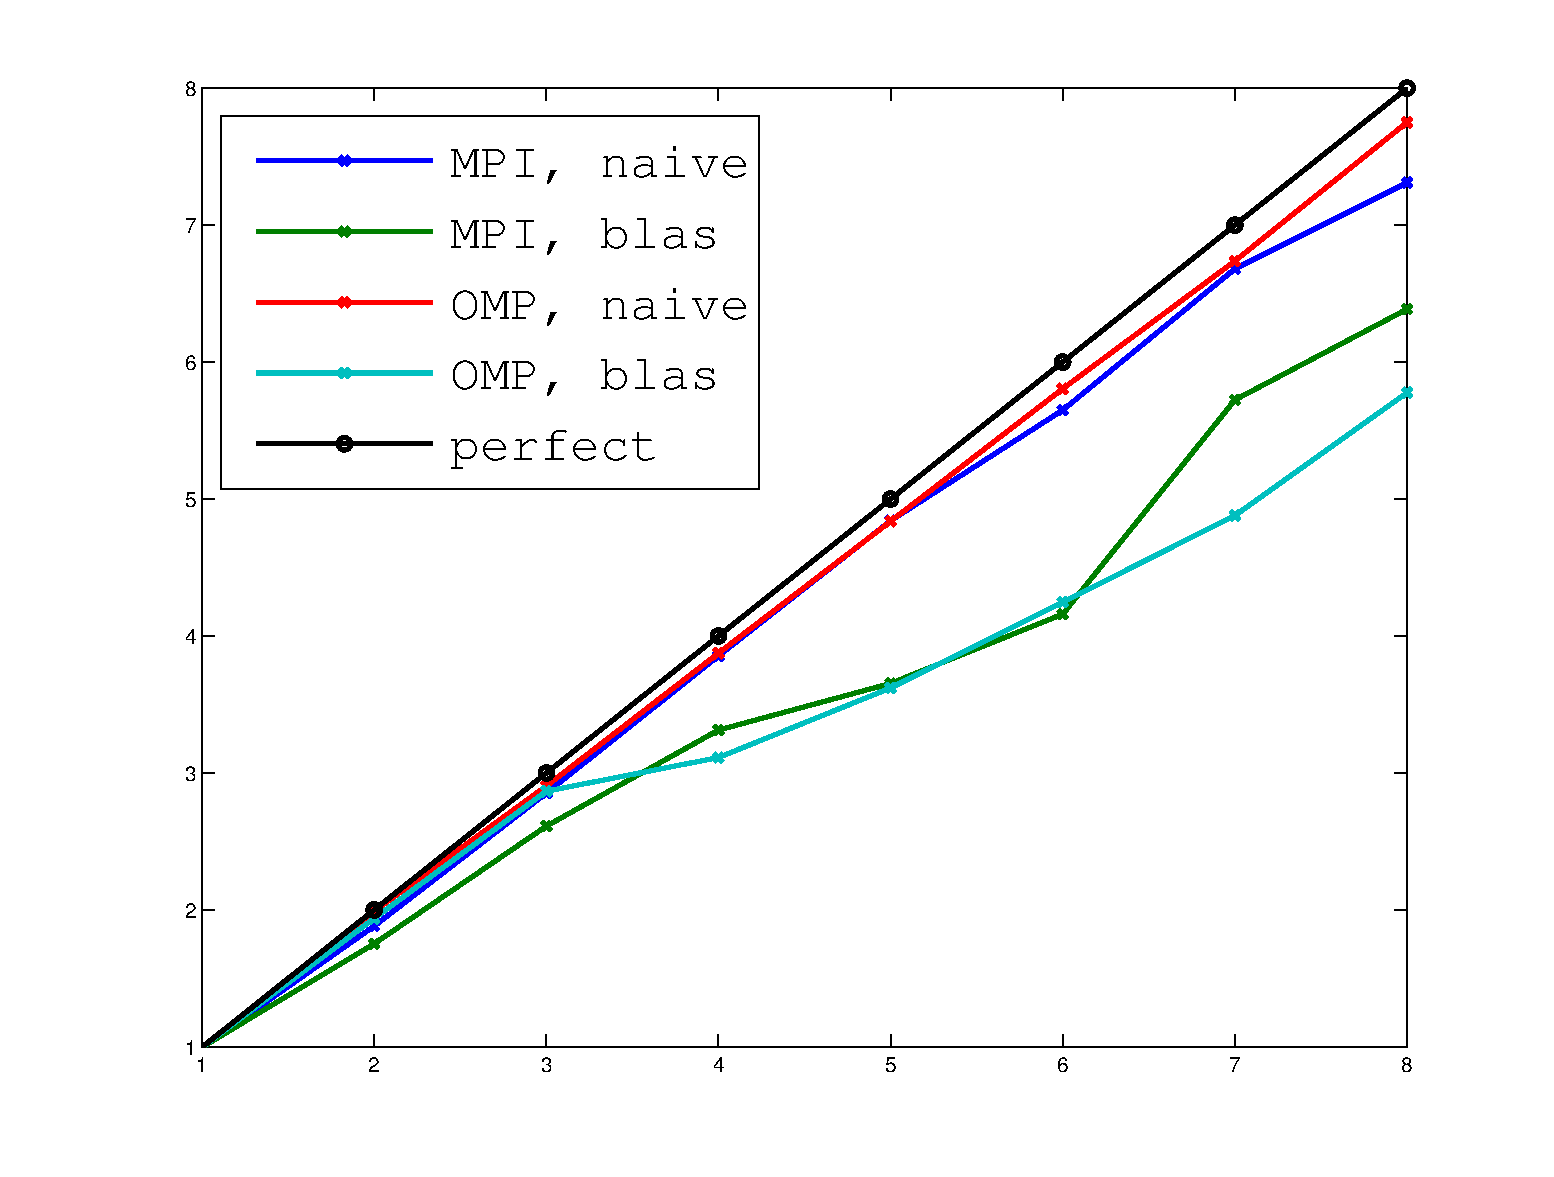
\includegraphics[width=8cm]{speedups}
    \end{center}
  \end{figure}
\end{frame}
\begin{frame}\frametitle{Using BLAS in the summing examples - results}
  \begin{itemize}
    \item Wall time with $N=16$ and $K=32768$: \\
      \ \\
      \begin{tabular}{r|c|c|c|c}
        \# t/P & Naive, OMP & BLAS, OMP & Naive, MPI & BLAS, MPI \\
        \hline
             1 & 0.009444 & 0.009095 & 0.010717 & 0.009361 \\
             2 & 0.020076 & 0.024310 & 0.007624 & 0.004478 \\
             4 & 0.015207 & 0.028780 & 0.006199 & 0.006233 \\
             8 & 0.007361 & 0.023888 & 0.005577 & 0.004677 
      \end{tabular}
  \end{itemize}
\end{frame}
\begin{frame}\frametitle{Using BLAS in the summing examples - speedups}
  With $N=16$ and $K=32768$:
  \begin{figure}[H]
    \begin{center}
      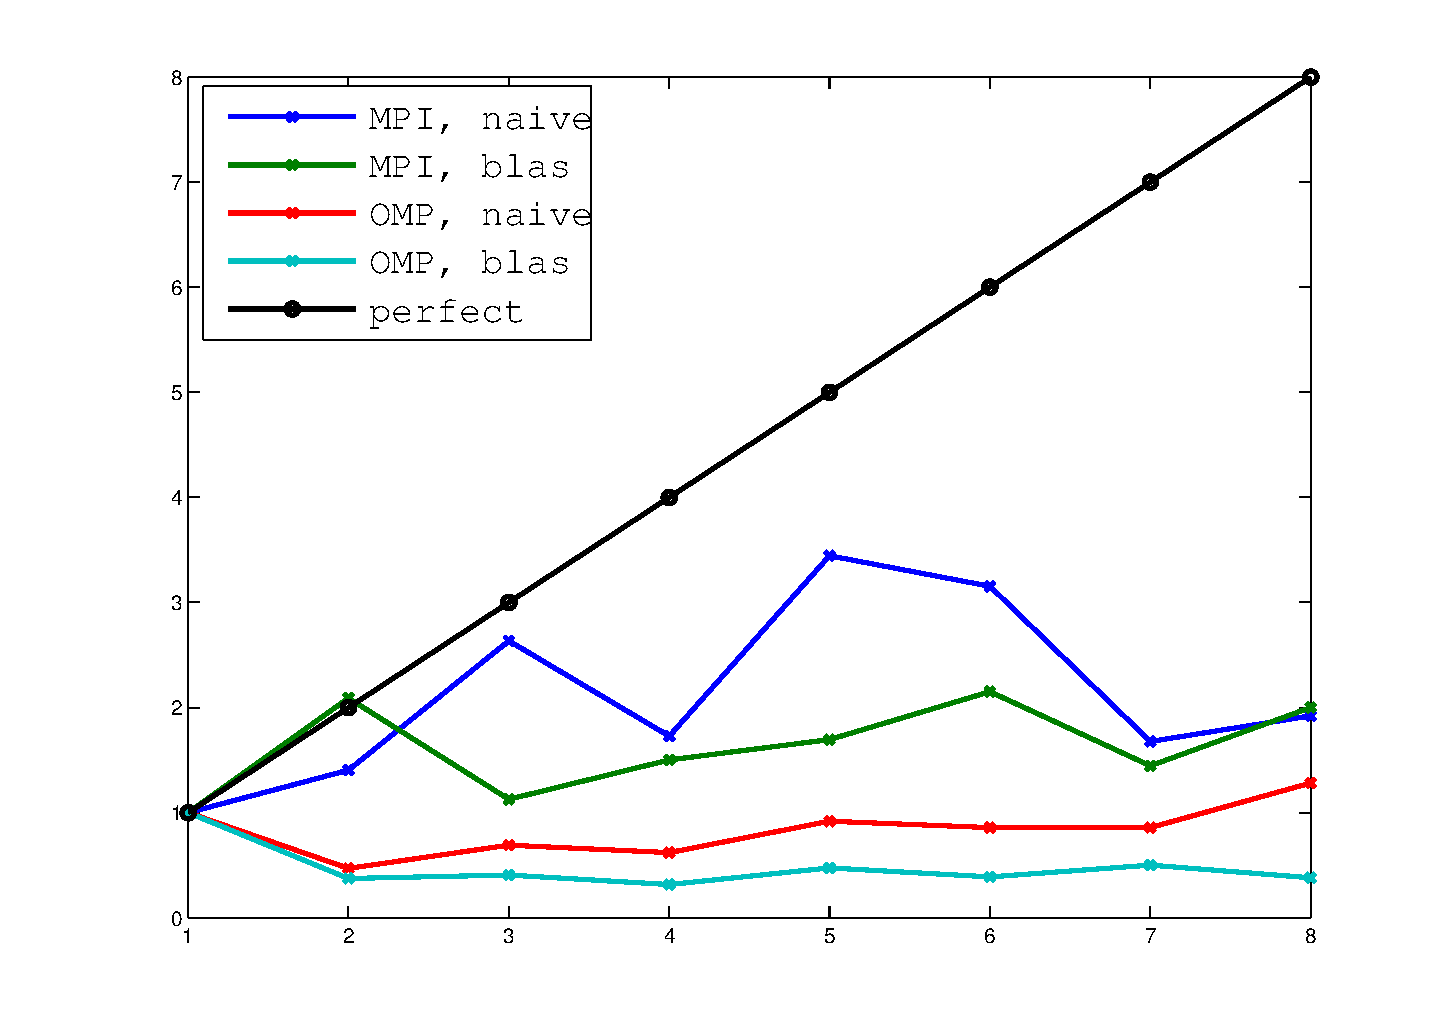
\includegraphics[width=8cm]{nospeedups}
    \end{center}
  \end{figure}
\end{frame}
\end{document}
